% sections/prefetching.tex
% TJ WILL WRITE THIS SECTION !!!

%This section explains the concept of link prefetching and discusses a possible usage of it as a defense mechanism against fingerprinting attacks on Tor.
A classifier used in a website fingerprinting attack can distinguish the differnce between two classes of packets when the difference is consisntent between them~\cite{Cai:2014kjb}. % "A systematic approach to ...", 2014
Thus, intuitively, a classifier would work the best if the difference in the same class is minimal and the difference among heterogeneous classes is high at the same time.
However, when variance among fingerprints in the same class is high, a classifier would not be able to characterize it clearly or at least the detection rate using the classifier would be low.
This is the basic idea of using prefetching as a defense mechanism; our conjecture is that we can use prefetching to manipulate the number and size of incoming and outgoing packets in order to increase the variance among packets in the same class.

This section explains the concept of link prefetching, discusses its effect on website fingerprints and argue its possible usage as a defense mechanism.

\subsection{Link Prefetching}

% introduction about link prefetching
Link prefetching is a HTML syntax that gives the web browser hints about which page the user is most likely to visit in a near future~\cite{fisher2003, fisher2004link}. 
The pages and resources to pre-fetch are specified in the web page so that the web browser can silently load them (or pre-fetch them) after an idle time.
Since the pre-fetch happens only after the page is fully loaded, it does not sacrifice the loading time of the requested web page.
Moreover, it can save the loading time for the pre-fetched pages and thus improve the user experience by caching the {\it future} contents.
It was first suggested by Mozilla Foundation in 2003 and supported by most modern browsers nowadays.

\iffalse %commented out
Once the web contents provider is reasonably certain about which links the users are most likely to visit next, it can improve the user experience by saving the loading time. 
Particularly, it is most effective if the content provider may be reasonably certain which links users are going to visit next.
Having been first suggested by Mozilla Foundation, it is adopted by most modern browsers nowadays.
Today's web browsers makes use of a specific syntax called \emph{pre-fetching}, which was proposed as a draft standard by Mozilla.
Using pre-fetching, browser can predicts documents likely to be visited by the user in the near future.
Therefore, based on the hint provided by pre-fetching a browser is able to fetch those documents a head of time.
In fact, it is the web page that provides a set of pre-fetching hints for the browser.
Then, loading the page and passing an idle time, the browser starts to pre-fetch and cache specified documents.
Needless to say, this mechanism improves efficiency.
\fi
% Insert a figure of "prefetch-network" which shows the network traffic.
% explain about how prefetching actually works 

The resources to prefetch can be simply specified in {\it HTML} using a {\tt link} tag~\cite{nottingham2010}.
For example, a {\tt link} tag {\tt <link rel="p\-refetch" href="/page2.html">} tells the browser to pre-fetch a {\it html} file named {\it page2.html}.
Resources other than a {\it HTML} web page can also be pre-fetched similarly using the same syntax.
There are also some variations for different types of prefetching -- DNS prefetching, which is specified as {\tt <link rel="dns-prefetch" ..>}, is supported by {\it Mozilla Firefox} and {\it Google Chrome}, and {\tt <link rel="prerender" ..>} also does the same job as {\tt prefetch} in {\it Google Chrome} and {\it Microsoft Internet Explorer}.

Figure~\ref{fig:network} illustrates how prefetching actually works in a browser ({\it Google Chrome}).
This page is set up arbitrarily by the authors to demonstrate link prefetching, and contains a link pre-fetch tag that specifies a big image (the image on the left side labeled as {\it prefetch}).
When the prefetching is off, this image shall be requested only when a user puts his mouse cursor on it (mouse over).
However, it can be seen on the network timeline (right bottom) that the image is pre-fetched right after loading the page.
This is indicated by a long blue bar on the second row for the file named ``{\it Very-high...}'', and it is long because the size of the file is relatively big ({\it 3.5 MB}) that it took a longer time to download.
Please also note that the time it took for loading the image when the user actually requested (by putting his mouse on it) was very short, because the image had already been pre-fetched that the browser merely loaded it from the cache (as shown in the {\it size} column on the fourth row).

\begin{figure*}[t]
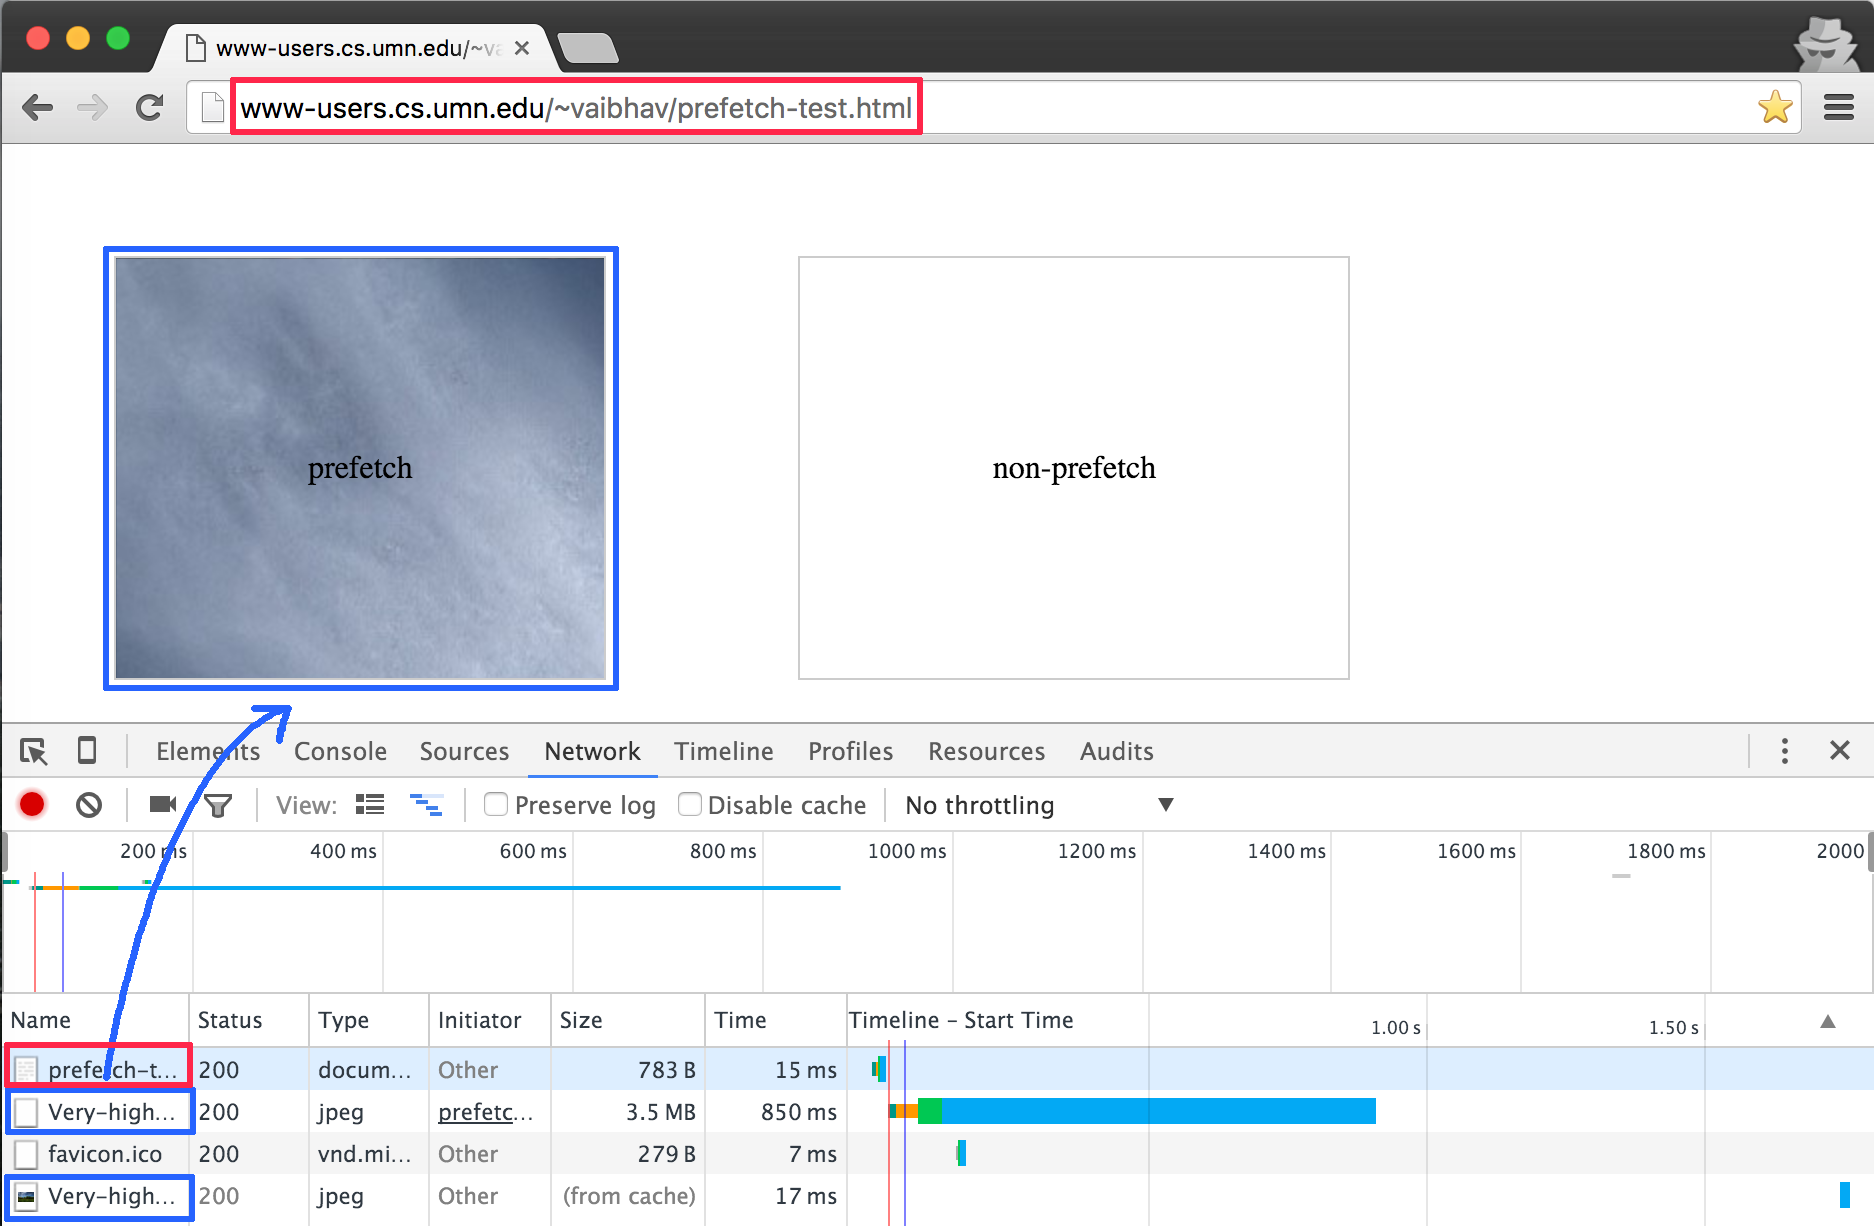
\includegraphics[width=\textwidth]{figures/prefetch-network-edited.png}
\centering
\caption{Network timeline showing pre-fetch}
\label{fig:network}
\end{figure*}


\subsection{The Effect of Prefetching on Website Fingerprint}
% cite some papers to describe about the features that are used for attacks,
% and explain why prefetching change the feature.
% Vaibhav says: put the intuition down 

% TODO: write few sentences as an intro
% We explained through an example how prefetching can affect the

% defenition of a fingerprint

%TODO: rewrite
\iffalse
Link prefetching obviously affects the traffic by sending additional request for prefetching items, and by prefetching those items after an idle time.
However, to what degree it affects the website fingerprint has not been studiedto the best of our knowledge.
This subsection first illustrates how the prefetching affects the number of packets being transferred as an example, and then discusses what features of fingerprint prefetching can possibly affect.
\fi


\subsubsection{An Example of prefetching packet sequence}

\begin{figure}[h]
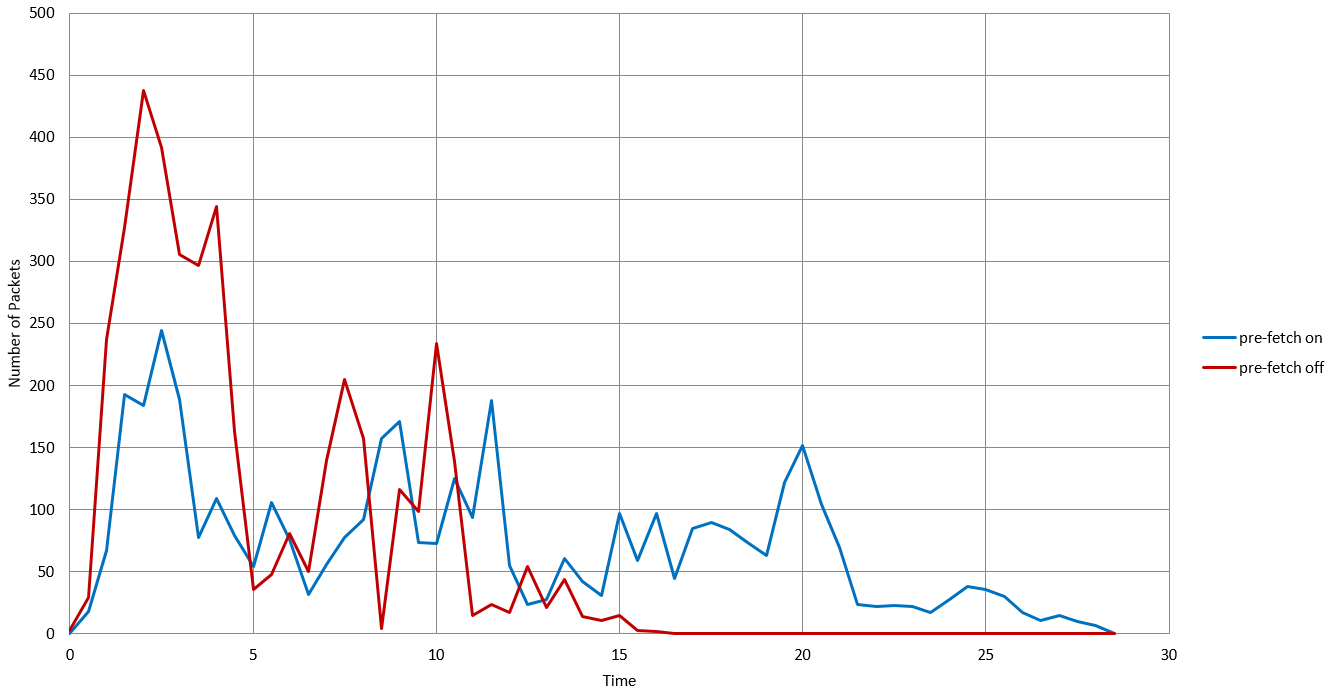
\includegraphics[width=0.95\columnwidth]{figures/prefetch.png}
\centering
\caption{A website fingerprint for pre-fetch on/off cases}
\label{fig:prefetch}
\end{figure}

%The idea of studying the effect of prefetching on Tor network is not new~\cite{something}.
Figure~\ref{fig:prefetch} illustrates a website fingerprint in terms of inter-packet timing, where the {\it x-axis} represents time in seconds and the {\it y-axis} represents the number of packets captured during a certain time interval ({\it 500 ms}).
The solid line depicts the packets captured while prefetching was enabled, and the dashed line depicts when the pre-fetch was disabled in the browser settings.
Both the cases are captured for the same web page, which is the first page of {\tt wired.com}.
However, the number of packets are slightly different for each case (4055 for the {\it off} case while 4218 for the {\it on} case), because the prefetch-on case obviously requests more resources for caching purpose. 
The elapsed time for loading the whole page was also different, but this variance is mainly due to the difference in network condition because all the packets are more scattered throughout time compared to the pre-fetch-off case.
When we ignore the speed difference, we can see that the four peaks of the two lines are roughly the same that if we capture the packets multiple times for the same website, we can characterize how the {\it fingerprint} of a specific website looks like.
Please note also that inter-packet timing is only one of many features for characterizing website fingerprint.


\subsection{Fingerprint Features}

Since all the traffic on Tor is encrypted, fingerprinting attacks blindly analyze a sequence of packets without knowing its contents, and extract {\it features} which characterizes a fingerprint.
The attacker then trains his/her classifier on multiple packet sequences from the set of website, for a set of features that attacker determined to use.
In this subsection, we summarize the definition of the four most popular features defined by Cai et. al.~\cite{Cai:2014kjb} to discuss the effect of prefetching on this features in the following subsection.

{\bf Packet Sequence}:
A packet sequence $P$ can be written as $P = \langle(t_1, l_1), (t_2, l_2), ..., (t_n, l_n)\rangle$ ~\cite{Cai:2014kjb}, where $t_i$ is the time relative to $t_0$ which is 0, and $l_i$ is the byte length of the $i$-th packet.

{\bf Unique Packet Lengths}: 
Most packets 
\begin{equation}
(\exists L \in P_l | L \notin P'_l ) \vee (\exists L \in P'_l | L \notin P_l)
\end{equation}

{\bf Packet Length Frequency}:
When $n_L(P_l)$ is the number of times packet length $L$ appears in $P_l$,
\begin{equation}
\exists L|n_L(P_l) \neq n_L(P'_l) \wedge n_L(P_l)>0 \wedge n_L(P'_l) >0
\end{equation}
In other words, $P$ and $P'$ have different packet length frequencies iff there exists a packet with length $L$ that appears different times in the two sequences.

{\bf Packet Ordering}:
When $M_l$ is the multiset of packet lengths in $P_l$ without ordering, two packet sequences $P$ and $P'$ have different packet ordering iff:
\begin{equation}
M_{ l }=M'_{ l }\wedge P_{ l }\neq P'_{ l }
\end{equation}

{\bf Interpacket Timing}:
\begin{equation}
\exists i, 1 \le i \le \mathit{min}(|P|, |P'|) : (P_t)_i \neq (P'_t)_i
\end{equation}


\subsubsection{The Effect of Prefetching on the Features}

Existing fingerprinting attacks extract {\it features} from a sequence of packets to characterize a distinct characteristic of a website.
The most popular features that have been used in the previous works for classification are unique packet lengths, packet length frequency, packet ordering, and interpacket timing.
Existing works on website fingerprinting considers a sequence
Packet lengths
Packet length frequency
Packet ordering.
Interpacket timing

Packet sequence.
